\begin{figure}[ht]
    \begin{subfigure}[t]{\textwidth}
        \caption{}
        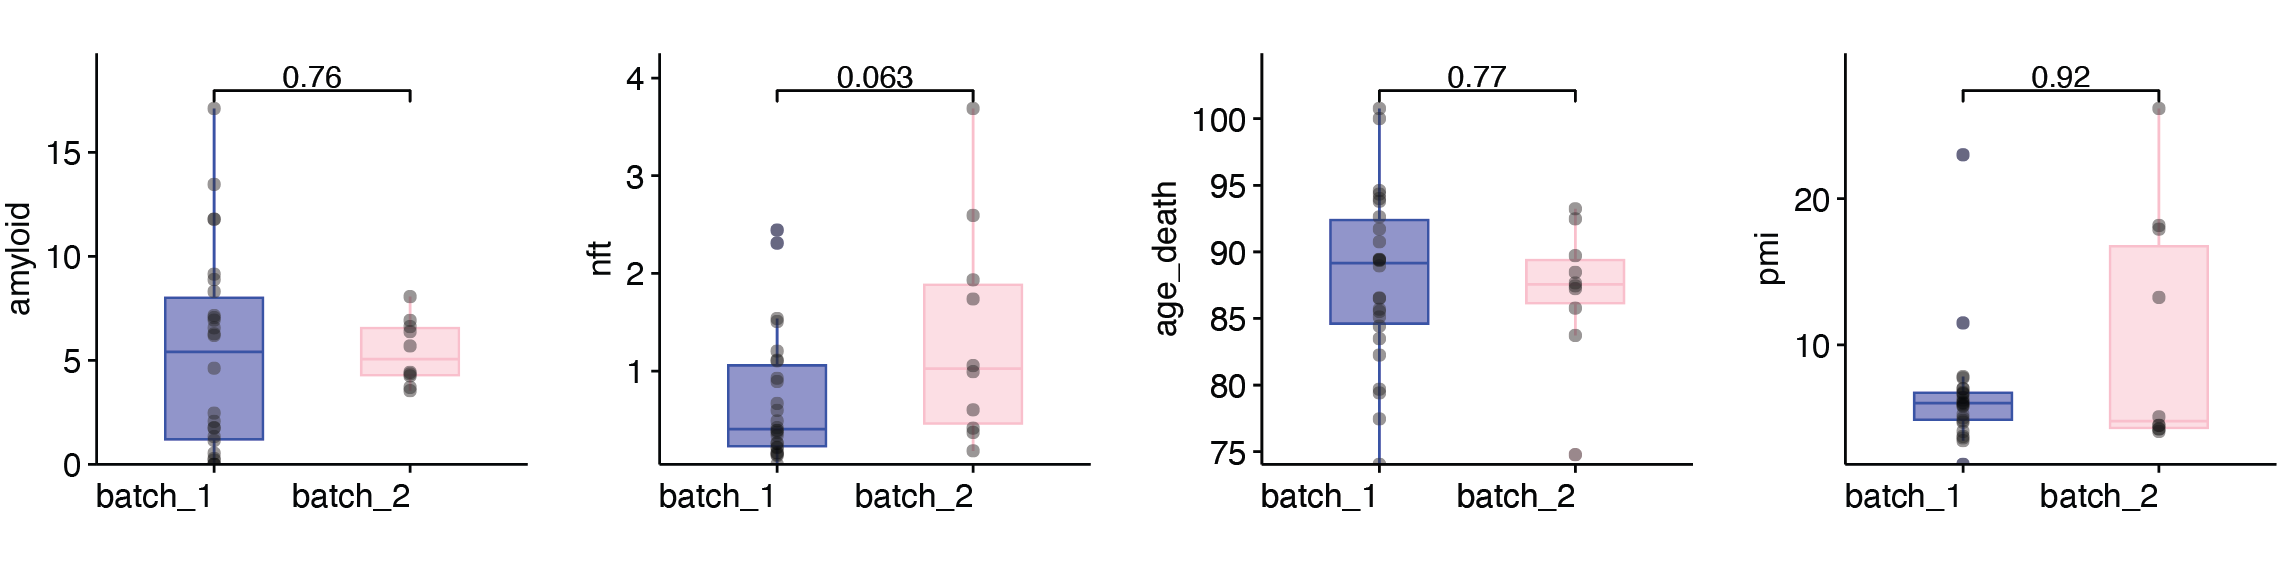
\includegraphics[width=\textwidth]{./extended_plots/seq_batch_cont.png}        
    \end{subfigure}
    \begin{subfigure}[t]{\textwidth}
        \caption{}
        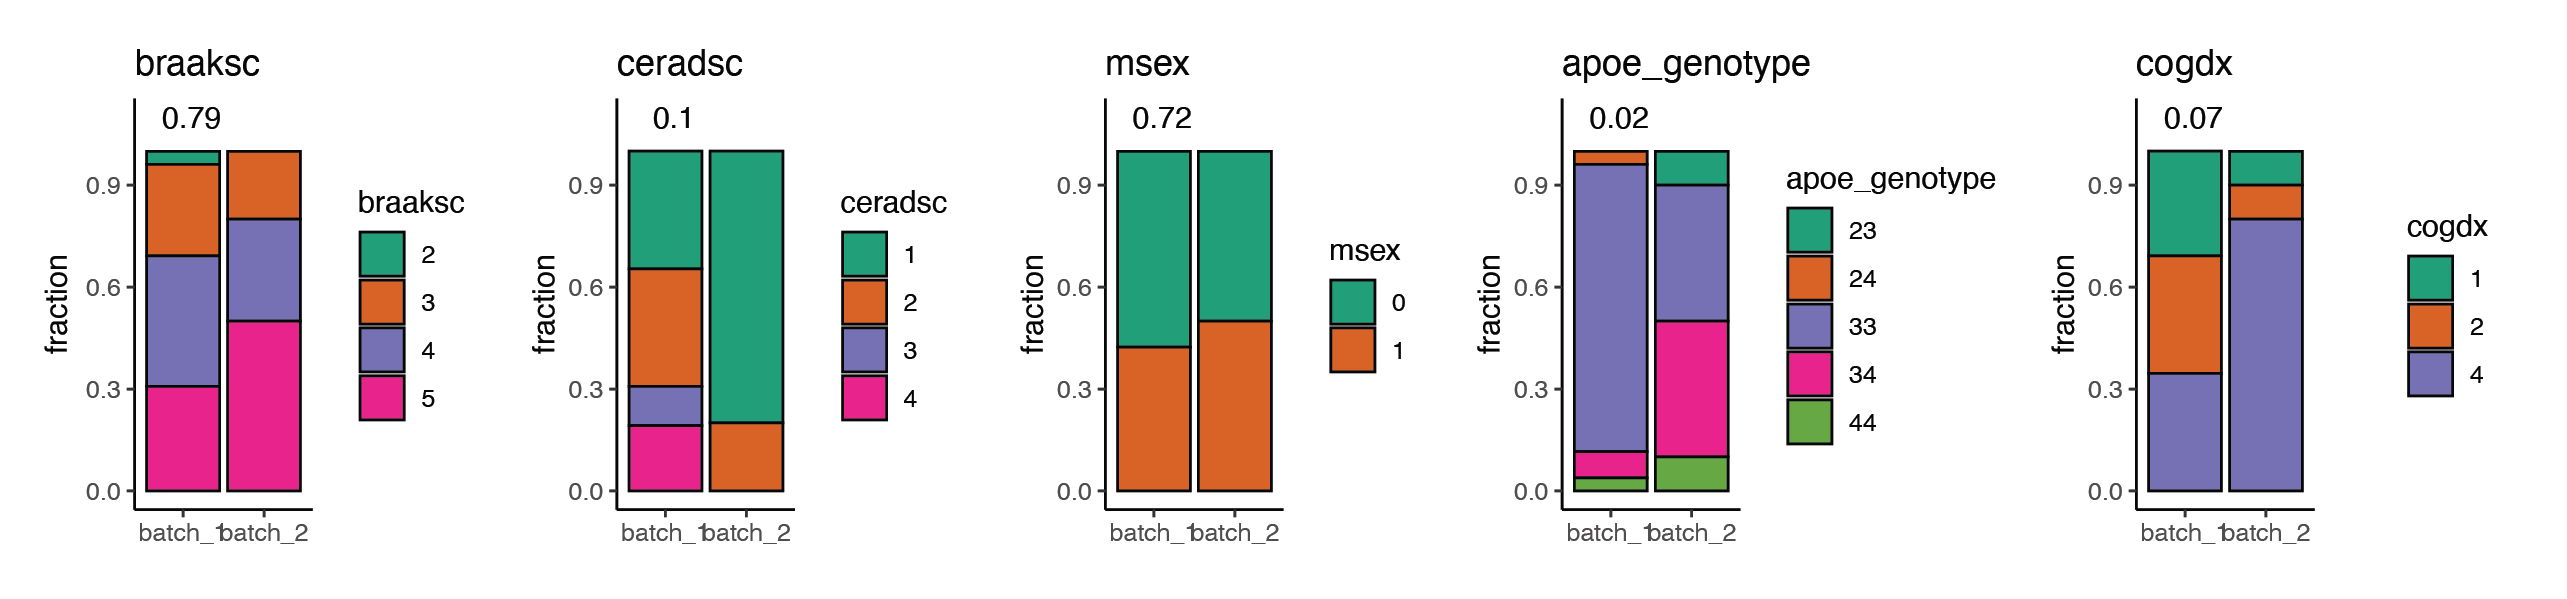
\includegraphics[width=\textwidth]{./extended_plots/seq_batch_cat.png}        
    \end{subfigure}  
    \begin{subfigure}[t]{.6\textwidth}
        \caption{}
        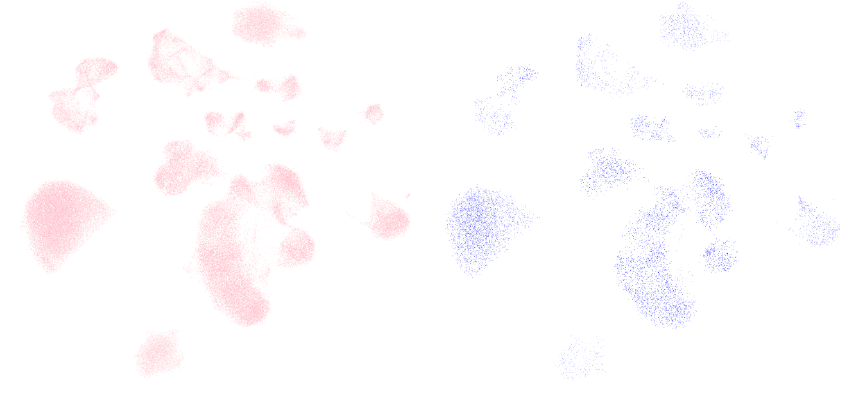
\includegraphics[width=\textwidth]{./extended_plots/seq_batch_projection.png}        
    \end{subfigure}   
    \begin{subfigure}[t]{.3\textwidth}
        \caption{}
        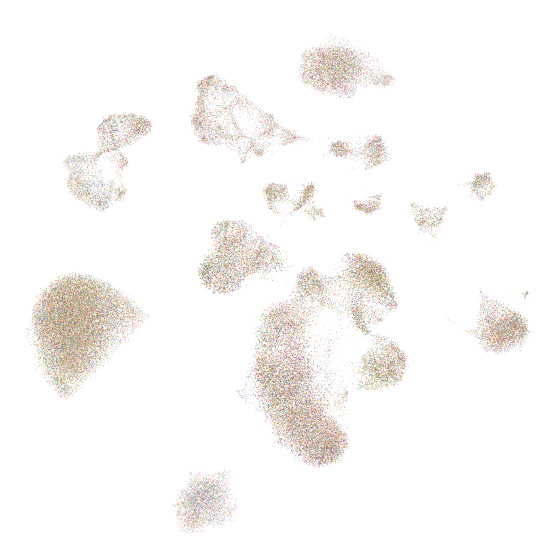
\includegraphics[width=\textwidth]{./extended_plots/projid_projection.png}        
    \end{subfigure}     
    \caption{
        \textbf{Overview of snRNA-sequencing Batch Correction, Data Quality, and Cell Type Annotations.}\\[1ex]
        (A,B) Distributions of continuous (A) and discrete (B) metadata variables by sequencing batch. 
        (C) Two-dimensional UMAP projection of snRNA-seq single cells from gene expression space, colored by batch 1 (pink) or batch 2 (blue) after all rounds of quality control. 
        (D) Two-dimensional UMAP projection of snRNA-seq single cells from gene expression space, colored by individuals of origin after all rounds of quality control. Each individual is indicated by a different color. 
        (E) Two-dimensional UMAP projections of individual cells from gene expression space, colored by Leiden clusters. 
        (F) Average marker gene expression (per-cluster mean log(fold-change)) for all marker genes for the cell type indicated along the x-axis. Log(fold-changes) are computed for the cluster of interest vs. all remaining clusters. Reference 1 (Table 2) marker genes were used. 
        (G) Cladogram visualizing subcluster relationships based on pairwise distances between per-cluster gene expression profiles. 
        (H) Average marker gene expression profiles (x-axis) per major cell type annotation (y-axis) for two marker gene references (Table 2). (I) Per-cell distribution of select marker gene expression by cell type. Y-axis indicates log counts. 
        (J) Median number of cells per cell type per individual. 
        (K) Cell type fraction by individual. (L,M) Individual-level gene expression correlations by cell type. For all panels, p-values for all continuous variables were computed by two-sided Wilcoxon rank sum test. P-values for all discrete variables were computed by two-sided Fisher’s exact test. For A, I, M boxes indicate per-condition dataset quartiles, and whiskers extend to the most extreme data points not considered outliers (i.e., within 1.5 times the interquartile range from the first or third quartile).
    }
    \label{fig:snRNA_quality_annotation}
\end{figure}